\chapter{Theory construction\label{cha:theory}}

This chapter presents a theory of how the GDR’s cultural diplomatic efforts through football were reflected in \textit{Neues Deutschland}. Although \textit{Neues Deutschland} was the mouthpiece of the Central Committee of the SED, it was the journalists who produced the articles published in the newspaper, thus controlling the narrative of how GDR footballers were presented.   The analyses from Chapters 2 and 3 provide the foundation upon which the proposed theory is constructed. The categories identified in Chapter 2 illuminate the actions taken by the journalists when reporting on the performances of the GDRNT. Chapter 3 provides the context in which the actions captured by the categories were applied. The proposed theory will then offer a model that shows the relationships between categories, explaining how \textit{Neues Deutschland} journalists were able to present GDRNT footballers through a cultural diplomatic lens.

\section*{\textit{Neues Deutschland} journalists}

Before presenting the theory, it is important to consider the people who wrote the articles published in \textit{Neues Deutschland} and any background information available on them. Of the 23 articles examined, Max Schlosser was attributed to have authored or co-authored 17. Horst Richter was a co-author of four articles, three with Max Schlosser and 1 with Eckhardt Galley (which was Galley’s only contribution in the period examined). Klaus Ullrich co-authored the final three articles with Max Schlosser in the period examined. Five articles had no attributed author and instead concluded the article with ‘ADN’, the acronym for the \textit{Allgemeiner Deutscher Nachrichtendiesnt} (General German News Service). The ADN was the state newsagency for the GDR and supplied content to GDR newspapers and television broadcasters (\cite{wilke1998}). Accessible information on the aforementioned journalists has proven difficult to come by. Klaus Ullrich was the only figure who had a substantial amount of accessible information written about him. Max Schlosser was \textit{Neues Deutschland’s} resident Oberliga\footnote{The Oberliga was the top division of the GDR football pyramid. It between 1948 and 1991 and was eventually absorbed into the West German football pyramid after re-unification.} reporter and Berliner FC Dynamo\footnote{Berliner FC Dynamo was a club that competed in the Oberliga competition of GDR football. It enjoyed the patronage of Erich Mielke, the long-time head of the \textit{Ministerium für Staatssicherheit} (The Ministry for State Security, or MfS), the organisation tasked with protecting the GDR from threats against socialism. For more information on the relationship between the MfS and football, refer to the chapter ‘‘Crooked champions’: the BFC problem’ in McDougall’s (\citeyear{mcdougall2014}) \textit{The People’s Game: Football, State and Society in East Germany}, pp. 223-244.} expert (\cite{kannowski1999}, p. 38). Unfortunately, no further information on Schlosser could be found. Eckhardt Galley was not only a journalist, but also served as a sports editor for \textit{Neues Deutschland} (\cite{landes2011}, p. 120).

Klaus Ullrich Huhn, writing under the pseudonym Klaus Ullrich, was the \textit{Sportchef des ND} (Head of Sports at \textit{Neues Deutschland}) from 1952 to 1990 (\cite{meyenfiedler2011}, p. 11). Huhn also moonlighted as a diplomat for GDR sports when other officials were not allowed to go abroad (\cite{meyenfiedler2011}). As evidenced by his co-authorship of the match reports from the World Cup Finals matches, along with the penultimate preparation match against England, Huhn can be seen as taking control of the reporting of important matches the GDRNT participated in. His responsibility as \textit{Sportchef des ND} played a role in this, as did his status as an \textit{Inoffizielle Mitarbeiter}\footnote{Briefly discussed in Chapter 1, \textit{Inoffizielle Mitarbeiter} (IM) were unofficial collaborators or co-workers who acted as the “eyes and ears” for the Stasi. They were in involved in all aspects of East German society and were tasked with reporting on their fellow citizens if they were acting against the interests of the state. Although determining the exact figure has proven to be difficult, the number of IM’s in the GDR was calculated to have hit a peak of 170000-180000 people in the 1980s. For more information see Fullbrook (\citeyear{fullbrook1995}, pp. 49-51) and Dennis (\cite{dennis2000}, pp. 212-215).} reporting on elite sportspersons for the Stasi (\cite{brinkbäumeretal1999}). The intersection of these roles demonstrates Huhn’s capacity to be \textit{linientreu} (loyal) to the goals of the SED and therefore the state. It also helps explain why ‘er habe so viel Spielraum gehabt, wie er wollte’ (he had as much leeway as he wanted) when producing content for \textit{Neues Deutschland} (\cite{landes2011}, p. 109).\footnote{Cornelia Landes interviewed Klaus Huhn as part of her Masters thesis in the Das Institut für Kommunikationswissenschaft und Medienforschung at Ludwig-Maximilians-Universität München (\cite{fiedlermeyen2011}, p. 20).} If we are to accept Huhn’s claim that he was not controlled in what he was allowed to publish in \textit{Neues Deutschland} (\cite{landes2011}, p. 107), then it could be assumed that Huhn dutifully performed his role in service to the state when attempting to ascribe desired qualities to GDR footballers in the match reports he published.

\section*{Ascriptive categories: Implication of an earlier wave of the \textit{Preußenwelle}}

Since the Constructivist Grounded Theory method requires the researcher to constantly move between data collection, data comparison, analysis and reflection, an initial hunch experienced earlier in the research journey has become fully realised. That is: \textit{Neues Deutschland} sports reporters were attempting to cultivate an East German cultural identity based on a Prussian heritage. Remarkably, the period from which the articles are sourced coincides with when the FRG recognised the GDR as a sovereign state. The two ascriptive categories, \textit{Associating Körperkultur with GDR footballers} and \textit{Associating militarism with GDR footballers}, both have implications that suggest links to a Prussian heritage.

\textit{Associating Körperkultur with GDR footballers} and \textit{Associating militarism with GDR footballers} could have been merged into one core category titled \textit{Associating Prussian heritage with GDR football}. However, I was careful not to ‘force preconceived ideas and theories’ onto the data and rather followed ‘leads that we \textit{define} in the data’ as Charmaz has suggested (\citeyear{charmaz2014}, p. 32, emphasis in original). Although the two categories are closely linked, there still exists a nuanced difference. \textit{Associating Körperkultur with GDR footballers} primarily interests itself with the coded references that catalogued how \textit{Neues Deutschland} journalists presented the physical qualities desired in GDR footballers. The coded references relating to \textit{Associating militarism with GDR footballers} demonstrate how \textit{Neues Deutschland} journalists applied the “football matches as battles” conceptual metaphor in their writing allowing them to emphasise specific behaviours found in GDR footballers’ performances. Put simply, \textit{Associating Körperkultur with GDR footballers} ascribed desired physical qualities to GDR footballers, whereas \textit{Associating militarism with GDR footballers} attributed desired mental qualities. If the two categories were prematurely merged during this research journey, the insight gained from the categories’ nuanced difference may have not been realised.

With Keil (\citeyear{keil2016}) and Colla (\citeyear{colla2019}) identifying the late 1970s and early 1980s as the arrival of the \textit{Preußenwelle} in the GDR, the period of the articles examined (1972-1974) suggests that evidence of an about-face in negative East German sentiment toward a Prussian heritage had already begun. While it may have not been as explicit as in September 1978, a time which saw Ingrid Mittenzwei publish \textit{Die zwei Gesichter Preußens}\footnote{In \textit{Die zwei Gesichter Preußens}, Ingrid Mittenzwei (\citeyear{mittenzwei1978}) made the argument that progressive periods in Prussia’s history had to be seen as integral parts of the GDR’s historical heritage. According to Keil, this was the first, clear shift in the GDR’s relationship with their Prussian heritage, moving from a negative perspective toward a positive recognition.  (\cite{keil2016}, p. 265).} in \textit{Forum}, the main journal of the \textit{Freie Deutsche Jugend} (Free German Youth), the articles examined demonstrate that there had been an already existing shift toward a positive perspective of the GDR’s Prussian heritage from \textit{Neues Deutschland} journalists. Whether this shift was consciously made, this thesis is unable to provide an answer. However, it does beg the question whether this shift in perspective was present in other circles of society. What can be ascertained from this study is that the \textit{Preußenwelle} may have arrived earlier than the late 1970s.

\section*{Ascriptive categories in use}

Chapter 3 has shown that the ascriptive categories’ coded references had a higher prevalence in the match reports where the GDRNT played in important fixtures (WCQ and WCF matches) or when the GDRNT recorded an emphatic win. Interestingly, matches where the GDRNT played against nations who were members of the NATO alliance did not elicit a higher proliferation of coded references relating to the ascriptive categories. This suggests that \textit{Neues Deutschland} journalists were more influenced by the importance of the match, rather than the political status of their opposition. It was in these important matches that \textit{Neues Deutschland} journalists saw the opportunity to positively present GDR footballers with the desired qualities one expected a representative of the GDR to have. With the opposition’s NATO membership having a negligible influence on when \textit{Neues Deutschland} journalists chose to ascribe these qualities, it becomes apparent that the motivation behind the presentation of these qualities did not come from the GDR’s position in Cold War politics, rather; it emanated from a desire to produce an East German cultural identity that was distinctive to the GDR. It is difficult to prove whether this distinctive East German cultural identity existed. This thesis only claims that \textit{Neues Deutschland} journalists attempted to \textit{produce} the narrative that it did exist.

The match reports covering the GDRNT’s WCF matches reveals how \textit{Neues Deutschland} journalists chose to present the GDR footballers in the most important matches the GDRNT would take part in. Not only were the GDRNT playing in the World Cup Finals for the first time, but they were also being held in the FRG. The coded references relating to the ascriptive categories appear when GDR footballers match the expectation of desired qualities with their performances. Ascriptive categories’ coded reference are all temporally situated within the present context of the match. Since the GDRNT’s performances elicited positive results, there exists a higher number of coded references related to the ascriptive categories. Huhn’s involvement in the publishing of the match reports, along with the alleged editorial freedom he enjoyed, suggests that attributing desired qualities with GDR footballers was a process used by \textit{Neues Deutschland} journalists when wanting to propagate the narrative of a distinctive East German cultural identity. Huhn and Schlosser may have seen the WCF matches as an opportune moment to highlight the cultural differences between the GDR and FRG, be they real or fictitious.

\section*{Evaluative categories in use}

Coded references relating to the evaluative categories occur when the performances of GDRNT footballers do not meet the expectation of desired qualities. The evaluative categories operate in reference to the ascriptive categories. Like the ascriptive categories, evaluative categories’ coded references are influenced by the context of the current match. The evaluative categories have different temporal characteristics, with some situated in the present, others moving from the past to the present or from the present to the future.

The evaluative categories relating to \textit{improvement} of the GDRNT’s performances operate across temporal axes. The coded categories relating to \textit{Highlighting the team’s ability to improve} and \textit{Highlighting the team’s need to improve} reference not only the current match which the article reports on, but they also refer to past or future matches. The contexts of the current match and referent past/future match influence the processes \textit{Neues Deutschland} journalists use when discussing issues related to performance improvement. Typically, matches of high importance (WCQ and WCF matches) elicit a greater use of these processes, evidenced by the higher frequency of coded references relating to the two \textit{improvement} categories. The matches of high importance could either be the current match being reported on, or a past or future match that the article refers to. Since coded references relating to \textit{improvement} categories appear regularly in most of the articles examined, it appears that \textit{Neues Deutschland} journalists held the perspective that the GDRNT could always improve and become a genuine power in world football.

\textit{Acknowledging a sub-standard performance from GDR footballers} contains coded references where \textit{Neues Deutschland} journalists recognised GDRNT performances as not displaying the expected desired qualities sought in GDR footballers. The category’s coded references are all temporally situated within the present context of the match. The ability for \textit{Neues Deutschland} journalists to be critical toward the GDRNT derives from the expectations placed on GDR footballers’ performances. If GDR footballers displayed the desired qualities in their performances, then the \textit{Neues Deutschland} journalists utilised the processes found in the ascriptive categories. If they did not display these qualities, then the alleged freedom afforded to \textit{Neues Deutschland} journalists allowed them to be critical of GDR footballers by employing the process captured by the \textit{Acknowledging a sub-standard performance from GDR footballers} category.

The process captured by the \textit{Avoiding being overtly critical} category suggests behaviours of self-censorship from \textit{Neues Deutschland} journalists. Unlike the coded references relating to \textit{Acknowledging a sub-standard performance} where \textit{Neues Deutschland} journalists were upfront in recognising flaws in the GDR footballer’s performances, \textit{Avoiding being overtly critical’s} related coded references reveal a different process of criticism from the journalists, where they both acknowledge the footballers’ deficiencies, but also are understanding of them. This suggests that \textit{Neues Deutschland} journalists were aware of the GDRNT’s mediocre standing in world football. It also highlights the journalists’ attempts to not present the GDRNT as totally deficient, but as a work in progress. The self-censorship is evidenced by the choice not to be overtly critical, but choosing to balance criticism with an understanding of the GDRNT’s performance capacity. This approach aligns with how Erich Honecker\footnote{Erich Honecker was the General Secretary of the SED and leader of the GDR between 1971 and 1989.} shifted perspectives of socialism in the GDR as ‘real existierenden Sozialismus’ (real existing socialism) (\cite{borowsky2002}).

\textit{Deflecting blame for poor performances} contains coded references that demonstrate when \textit{Neues Deutschland} journalists shifted blame for poor performances onto external factors. The process captured by this category sees \textit{Neues Deutschland} journalists absolving the GDRNT from blame when their performances do not meet the standards expected of them. This process also works to present a narrative of GDRNT footballer facing adversity, evidenced by the references made from \textit{Neues Deutschland} journalists on poor pitch conditions, having players injured due to opposition challenges or match regulations prohibiting the use of foot equipment which GDR footballers were accustomed to.

\section*{Theoretical model}

The relationships between the ascriptive and evaluative categories have been ordered into a theoretical model that displays how \textit{Neues Deutschland} journalists reported the performances of the GDRNT in the articles they published. The ascriptive categories capture the processes employed by \textit{Neues Deutschland} journalists when attempting to present GDR footballers as having the desired qualities associated with a distinctive East German cultural identity. The evaluative categories use the ascriptive categories as a reference point. They capture the processes employed by \textit{Neues Deutschland} journalists when GDRNT performances did not reach the standard expected of them outlined in the ascriptive categories.

\begin{figure}[h]
\caption{Theoretical model}
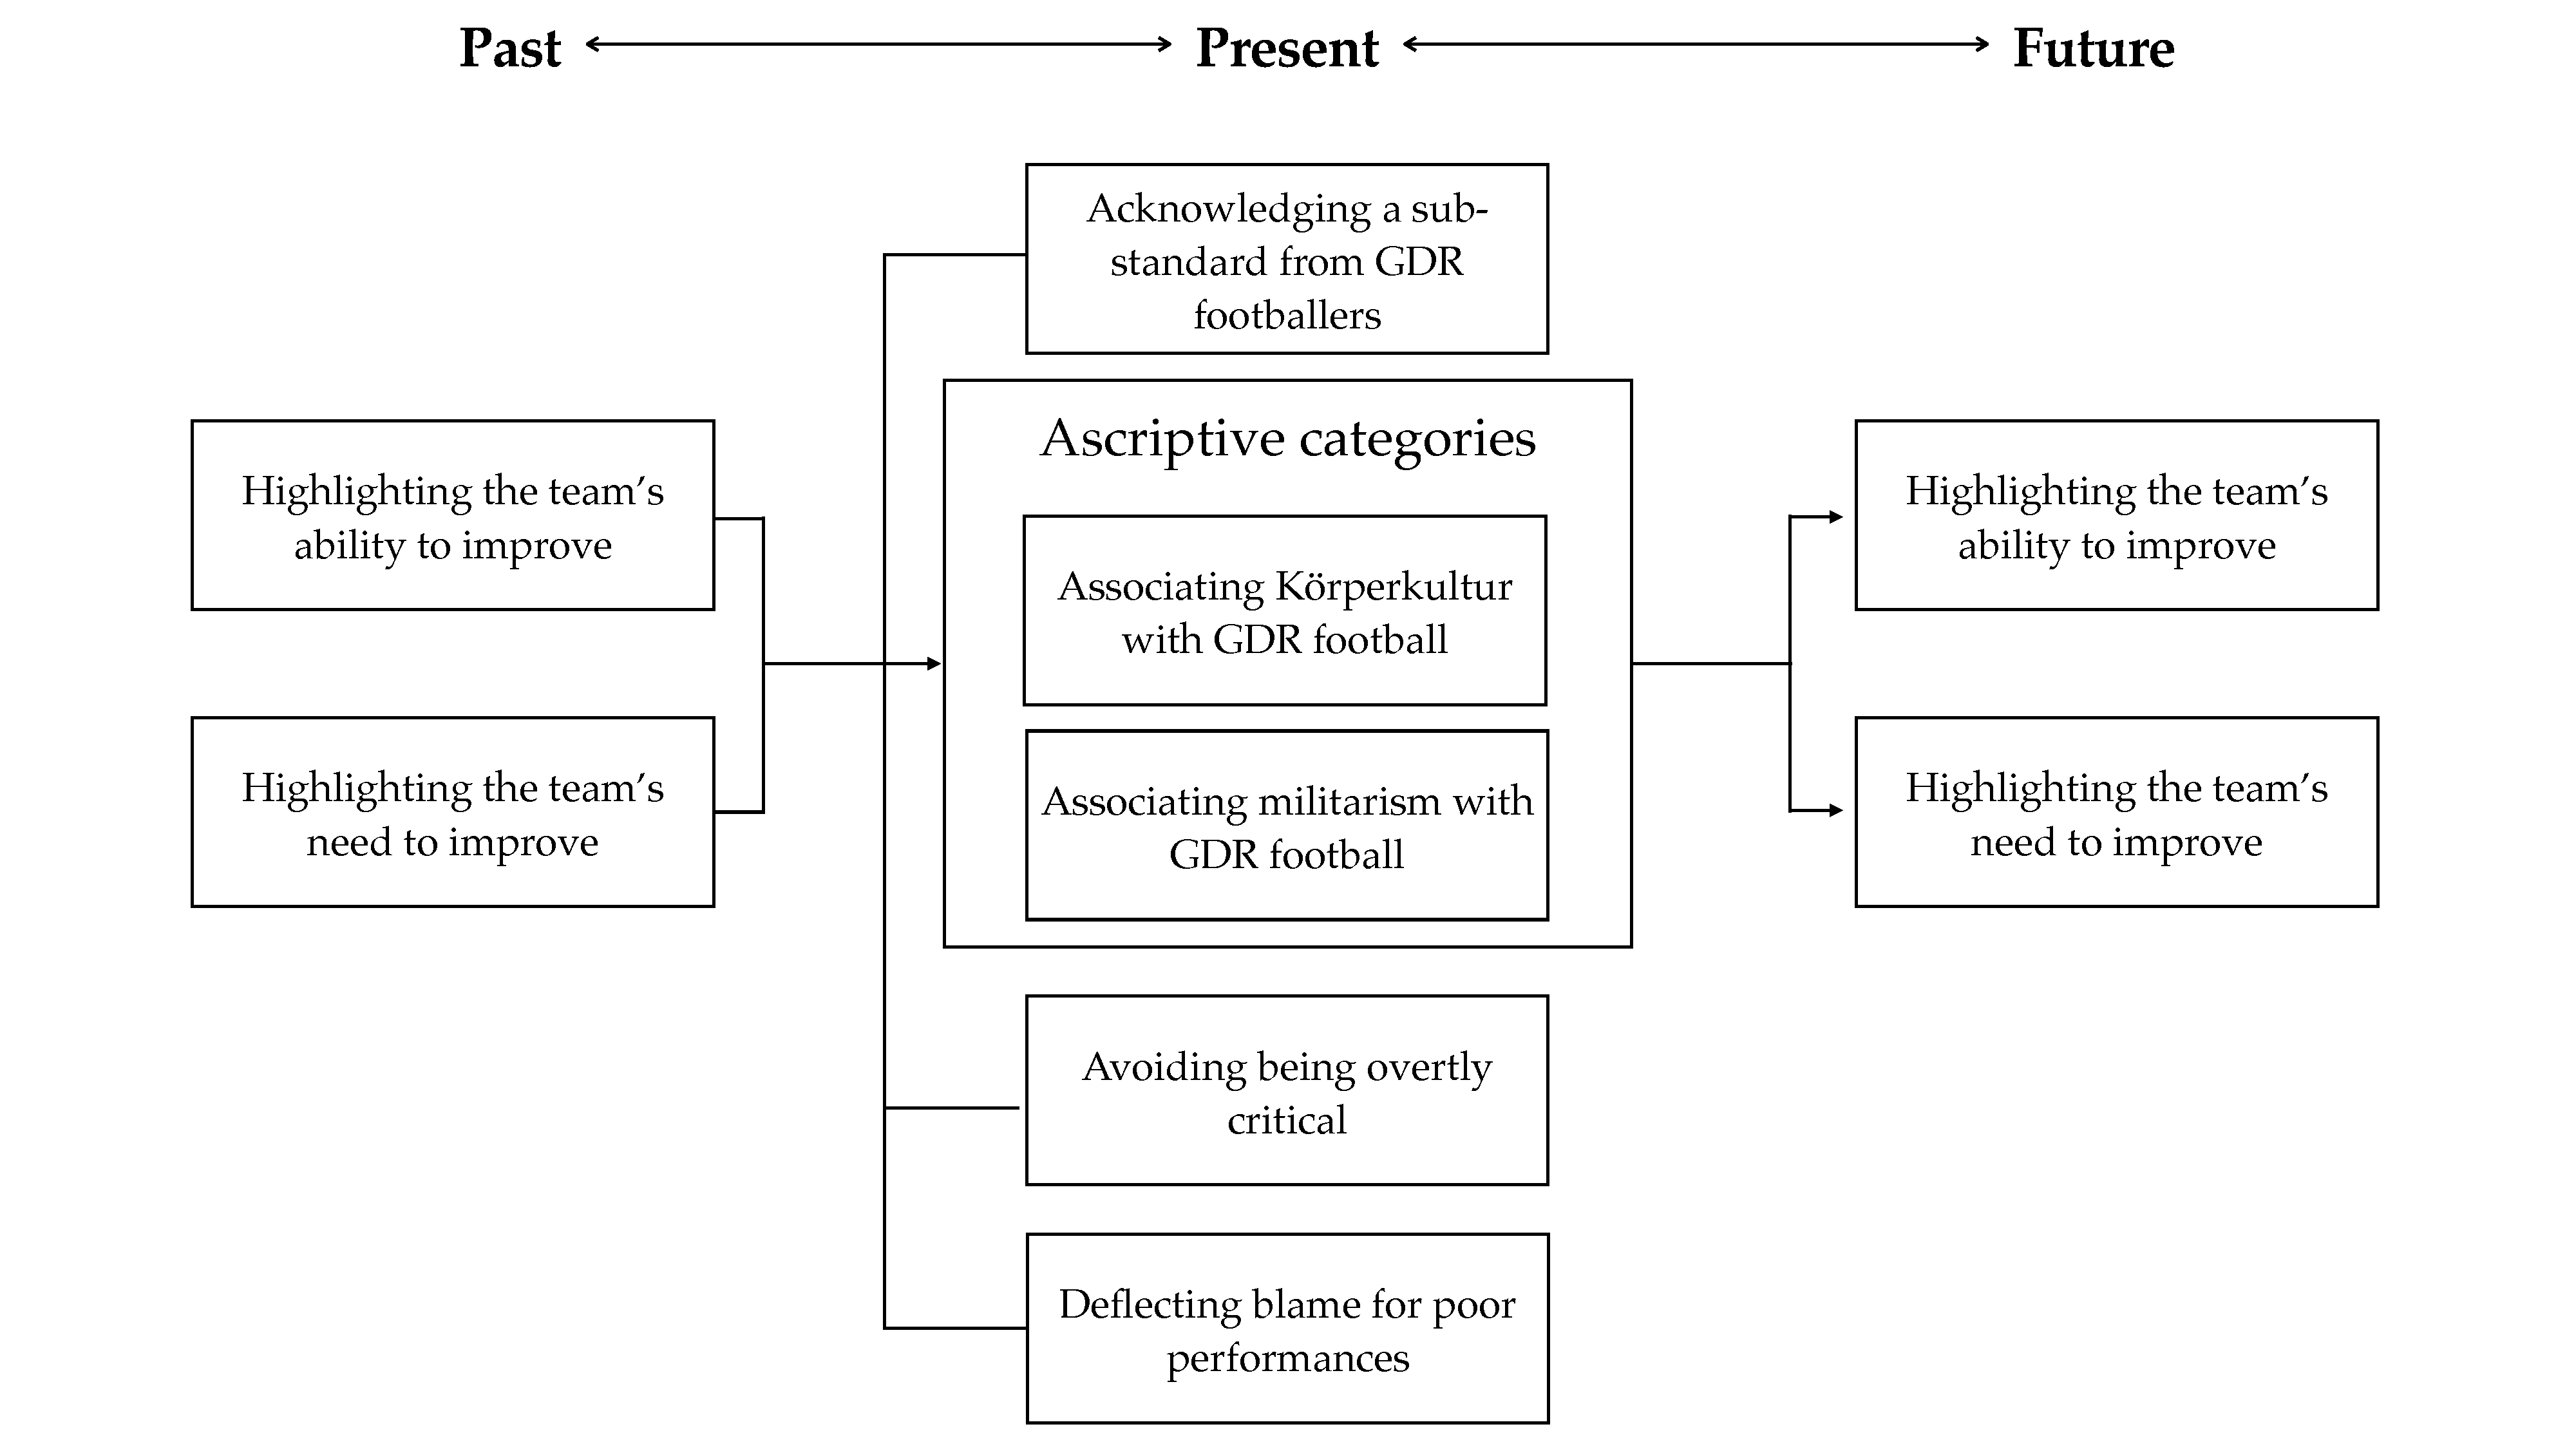
\includegraphics[width=\textwidth]{mres/images/figure 4.1.pdf}
\centering
\label{fig:fig4.1}
\end{figure}

\section*{Conclusion}

The practices of cultural diplomacy were reflected when the performances of the GDRNT reached an exemplary level, allowing \textit{Neues Deutschland} journalists to ascribe desired qualities associated with a distinctive East German cultural identity. This cultural identity was not influenced by the greater geopolitical landscape of the Cold War, but rather from the desire to see the GDR as a sovereign state with its own cultural heritage. This desire was possibly motivated by the GDR’s newfound recognition from the FRG as a sovereign state. This study suggests that the re-embracing of Prussian heritage within produced narratives of East German cultural identity predates the arrival of the \textit{Preußenwelle} in the late 1970s and 1980s. With German reunification seeming unlikely during the time period analysed, presenting the narrative of an existent, distinctive East German cultural identity was of paramount importance to those involved in the running of the GDR. This thesis does not (and cannot) prove whether this East German cultural identity imbued with Prussian heritage existed. It only demonstrates that there were attempts to \textit{produce} a narrative where the cultural identity did exist. The produced narrative is evident in how \textit{Neues Deutschland} journalists reflected the cultural diplomatic efforts of the GDR in the newspaper articles reporting on the performances of the GDRNT. 